
\chapter{Evaluation}
\label{chap:evaluation}

It is widely accepted that text simplification can be performed by \emph{splitting}, \emph{deletion} and \emph{paraphrasing} (\cite{feng}). The splitting operation breaks down a long
sentence into shorter ones. Deletion gets rid of unimportant parts of a sentence. The paraphrasing operation includes reordering, lexical substitutions and syntactic transformations (\cite{xu-etal-2016-optimizing}). The best method for determining the quality of simplification is through human evaluation. Traditionally, a simplified output is judged in terms of grammaticality, meaning preservation and simplicity. For training and comparing models, the most commonly used automatic metrics are:

\begin{itemize}
    \item \emph{BLEU}, to assess an extent to which the output differs from the references;
    \item \emph{SARI}, to evaluate the quality of the output by comparing it against the input and references;
    \item \emph{FKGL}, to estimate the readability of the output.
\end{itemize}

\section{BLEU}
\label{sec:bleu}

BLEU (\emph{Bilingual Evaluation Understudy}) is a precision-oriented metric that estimates the proportion of \textit{n}-gram matches between a system’s output and a reference (\cite{papineni-etal-2002-bleu}). It was one of the first metrics which had shown a high correlation with human judgments of quality and remains one of the most popular automated, inexpensive and language-independent metrics.

BLEU uses a modified precision to compare a candidate translation against multiple references. The reason for the modification is that machine translation systems can generate more words than there are in the references. A simple precision measure sums the number of candidate \textit{n}-grams which appear in any reference and then divides it by the total number of \textit{n}-grams in the candidate translation. This may result in a poor translation with high precision (Table \ref{tab:poor-translation}).

\begin{table}[h]
\centering
\begin{tabular}{ll}
\hline
Candidate: & {\fontfamily{pcr}\selectfont the the the the the the the.} \\
Reference 1: & {\fontfamily{pcr}\selectfont The cat is on the mat.} \\
Reference 2: & {\fontfamily{pcr}\selectfont There is a cat on the mat.} \\
\hline
\end{tabular}
\caption{Example of poor machine translation output with high precision. Source: \cite{papineni-etal-2002-bleu}.}
\label{tab:poor-translation}
\end{table}

\bigskip
All seven words in the candidate translation appear in the references. Thus a unigram simple precision is:

\[P=\frac{m}{w_t}=\frac{7}{7}=1\]

where $m$ is a number of words from the candidate found in the references, and $w_{t}$ is the total number of words in the candidate. This is an example of a perfect score given for a poor translation.

A simple modification solves this issue. To calculate modified unigram precision we first count the maximum number of times a word occurs in any single reference translation. Next, we clip the total count of each candidate word by its maximum
reference count $Count_{clip} = min(Count, Max\_Ref\_Count)$, add these clipped counts up, and divide by the total (unclipped) number of candidate words (\cite{papineni-etal-2002-bleu}). In the above example, the modified unigram precision score would be:

\[P=\frac{min(Count, Max\_Ref\_Count)}{w_t}=\frac{min(7, 2)}{7}=\frac{2}{7}\]

The modified \textit{n}-gram precision is computed similarly for any \textit{n}: all candidate \textit{n}-gram counts and their corresponding maximum reference counts are collected. The candidate counts are clipped by their corresponding reference maximum value, summed, and divided by the total number of candidate \textit{n}-gram. The \textit{n} which has the highest correlation with human judgments was found to be 4. The unigram scores account for the adequacy of the translation, while the longer \textit{n}-gram account for the fluency (\cite{papineni-etal-2002-bleu}).

One of the problem with the modified \textit{n}-gram precision is that it fails to enforce the proper translation length. A possible candidate translation for the above example might be {\fontfamily{pcr}\selectfont the cat} and the modified unigram precision would be:

\[P=\frac{1}{2} + \frac{1}{2}=1\]

To overcome this problem a \emph{multiplicative brevity penalty factor} is used. With the brevity penalty in place, a high-scoring candidate translation must match the reference translations in length, in word choice, and in word order (\cite{papineni-etal-2002-bleu}). If the total length of the translation corpus $c$ is less then or equal to the total length of the reference corpus $r$, the brevity penalty is decaying exponential with $r/c$: 

\[BP=e^{1-\frac{r}{c}}\]

Thus BLEU score is the geometric mean of the test corpus’s modified precision scores multiplied by an exponential brevity penalty factor. Geometric average of the modified \textit{n}-gram precisions, $p_{n}$, is calculated using \textit{n}-grams up to $N$ and positive weights $w_{n}$ summing to 1:

\[BLEU=BP \times \exp(\sum_{n=1}^{N}w_n \log p_n)\]

Despite being widely used and considered to be an informative metric for text-to-text generation, including text simplification, BLEU is not well suited for assessing simplicity from a lexical point of view (\cite{xu-etal-2016-optimizing}). Moreover, BLEU often negatively correlates with simplicity, essentially penalizing simpler sentences (\cite{sulem-etal-2018-bleu}).

\section{SARI}

\emph{SARI}, introduced by \cite{xu-etal-2016-optimizing}, compares system output against the references and against the input sentence. It measures how the simplicity of a sentence was improved based on the words added, deleted and kept by the system (fig. \ref{fig:sari}).

\begin{figure}[h]
    \centering
    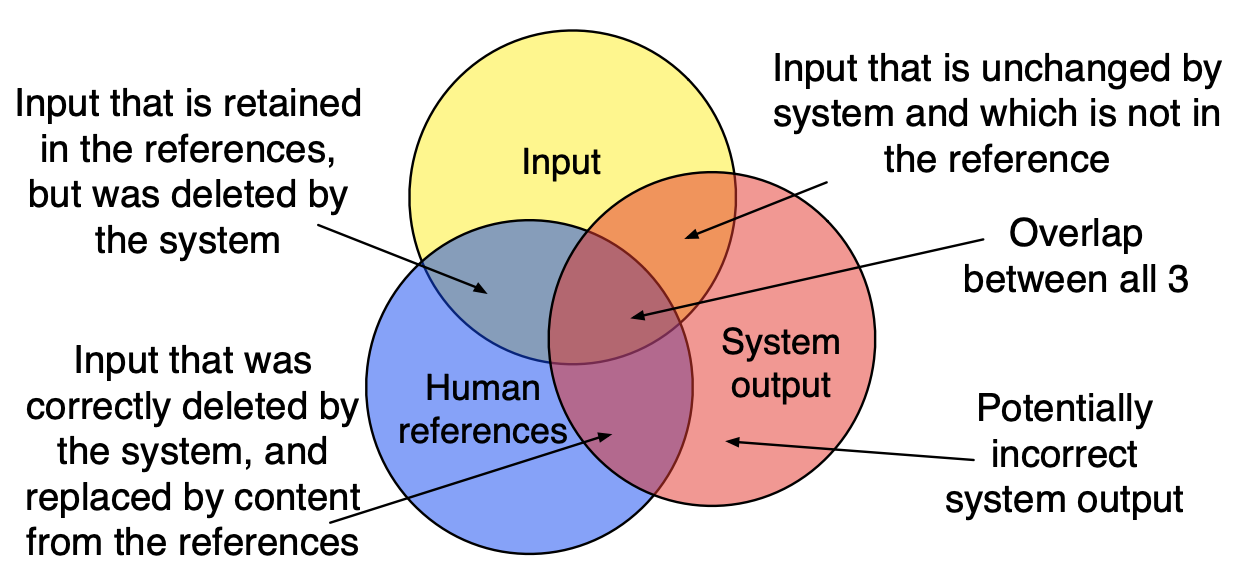
\includegraphics[width=10cm]{Images/sari.png}
    \caption{Metrics that evaluate the output of monolingual text-to-text generation systems. The different regions of this Venn diagram are treated differently with the SARI metric. Source: \cite{xu-etal-2016-optimizing}.}
    \label{fig:sari}
\end{figure}

\bigskip
SARI rewards addition operations, where system output $O$ was not in the input $I$ but occurred in any of the references $R$, i.e. $O\cap \bar{I} \cap R$. We define \textit{n}-gram precision $p(n)$ and recall $r(n)$ for addition operations as follows (\cite{xu-etal-2016-optimizing}):

\begin{equation}
p_{add}(n)=\frac{\sum_{g \in O} \min \left(\#_{g}(O \cap \bar{I}), \#_{g}(R)\right)}{\sum_{g \in O} \#_{g}(O \cap \bar{I})} 
\end{equation}

\begin{equation}
r_{add}(n) =\frac{\sum_{g \in O} \min \left(\#_{g}(O \cap \bar{I}), \#_{g}(R)\right)}{\sum_{g \in O} \#_{g}(R \cap \bar{I})} 
\end{equation}

where $\#g(\cdot)$ is a binary indicator of occurrence of \textit{n}-grams $g$ in a given set and

\setlength\extrarowheight{10pt}
\hspace*{3em}
\begin{tabular}{l}
$\#_{g}(O \cap \bar{I})=\max \left(\#_{g}(O)-\#_{g}(I), 0\right)$ \\
$\#_{g}(R \cap \bar{I})=\max \left(\#_{g}(R)-\#_{g}(I), 0\right)$
\end{tabular}

\bigskip
Example below (Table \ref{tab:sari-example}) demonstrates how the addition of word \textit{now} is rewarded in both $p_{add}(n)$ and $r_{add}(n)$, but the addition of \textit{you} in \textit{Output 1} is penalized in $p_{add}(n)$.

\setlength\extrarowheight{0pt}
\begin{table}[h]
\centering
\begin{tabular}{ll}
\hline
Input: & {\fontfamily{pcr}\selectfont About 95 species are currently accepted.} \\
Reference 1: & {\fontfamily{pcr}\selectfont About 95 species are currently known.} \\
Reference 2: & {\fontfamily{pcr}\selectfont About 95 species are now accepted.} \\
Reference 3: & {\fontfamily{pcr}\selectfont 95 species are now accepted.} \\
Output 1: & {\fontfamily{pcr}\selectfont About 95 you now get in.} \\
Output 2: & {\fontfamily{pcr}\selectfont About 95 species are now agreed.} \\
Output 3: & {\fontfamily{pcr}\selectfont  About 95 species are currently agreed.} \\
\hline
\end{tabular}
\caption{Example of sentence simplifications for SARI calculation. Source: \cite{xu-etal-2016-optimizing}.}
\label{tab:sari-example}
\end{table}

\bigskip
The $SARI$ scores for these outputs are $0.2683$, $0.7594$, and $0.5890$ respectively. The BLEU scores are $0.1562$, $0.6435$, and $0.6435$. BLEU is unable to separate \textit{Output 2} and \textit{Output 3} because matching any of the references is rewarded in the same way.

SARI rewards keep operation, where \textit{n}-grams are retained in both output and references. Number of such references matters. It bears in mind that some words or phrases don't require simplification:

\begin{equation}
p_{keep}(n)=\frac{\sum_{g \in I} \min \left(\#_{g}(I \cap O), \#_{g}I \cap R')\right)}{\sum_{g \in I} \#_{g}(I \cap O)} 
\end{equation}

\begin{equation}
r_{keep}(n) =\frac{\sum_{g \in I} \min \left(\#_{g}(I \cap O), \#_{g}(I \cap R')\right)}{\sum_{g \in I} \#_{g}(I \cap R')} 
\end{equation}

where

\setlength\extrarowheight{10pt}
\hspace*{3em}
\begin{tabular}{l}
$\#_{g}(I \cap O)=\min \left(\#_{g}(I), \#_{g}(O)\right)$ \\
$\#_{g}(I \cap R')=\min \left(\#_{g}(I), \#_{g}(R)/r\right)$
\end{tabular}

\bigskip
$R'$ indicates the \textit{n}-gram count over $R$ with fractions. In the above example (Table \ref{tab:sari-example}) 2 out of the total $r=3$ references contain the word {\fontfamily{pcr}\selectfont  about}, thus its count is weighted by 2/3.

For deletion, SARI calculates precision only. Deleting too many words decreases readability far more than not deleting:

\begin{equation}
p_{del}(n)=\frac{\sum_{g \in I} \min \left(\#_{g}(I \cap \bar{O}), \#_{g}I \cap \bar{R'})\right)}{\sum_{g \in I} \#_{g}(I \cap \bar{O})} 
\end{equation}

where

\setlength\extrarowheight{10pt}
\hspace*{3em}
\begin{tabular}{l}
$\#_{g}(I \cap \bar{O})=\max \left(\#_{g}(I) - \#_{g}(O), 0\right) $ \\
$\#_{g}(I \cap \bar{R'})=\max \left(\#_{g}(I) - \#_{g}(R)/r, 0\right)$
\end{tabular}

\bigskip
Final SARI score calculates arithmetic average of \textit{n}-gram precisions and recalls:

\begin{equation}
SARI=d_{1} F_{add}+d_{2} F_{keep}+d_{3} P_{del}
\end{equation}

where 

\setlength\extrarowheight{12pt}
\hspace*{3em}
\begin{tabular}{l}
$d_{1}=d_{2}=d_{3}=1/3$ \\
$P_{operation}=\frac{1}{k} \sum_{n=[1, \ldots, k]} p_{operation}(n)$ \\
$R_{operation}=\frac{1}{k} \sum_{n=[1, \ldots, k]} r_{operation}(n)$ \\
$F_{operation}=\frac{2 \times P_{operation} \times R_{operation}}{P_{operation}+R_{operation}}$ \\
$operation \in[del, keep,add]$
\end{tabular}
\setlength\extrarowheight{0pt}

\bigskip
where $k$ is the highest \textit{n}-gram order.

\section{BLEU vs SARI}

\cite{xu-etal-2016-optimizing} and \cite{wubben-etal-2012-sentence} showed that $BLEU$ does not demonstrate significant correlation with the simplicity scores rated by humans. In contrast, SARI achieves a much better correlation with human evaluations of simplicity. On the other hand, BLEU has a higher correlation on grammaticality and meaning preservation. BLEU gives a higher score to an output that is not too short and contains only \textit{n}-grams that occur in references. When applied to monolingual tasks like simplification, it does not take into account any differences between the input and the references. Whereas SARI considers both precision and recall looking at the differences between the references and the input (\cite{xu-etal-2016-optimizing}).

\begin{figure}[h]
    \centering
    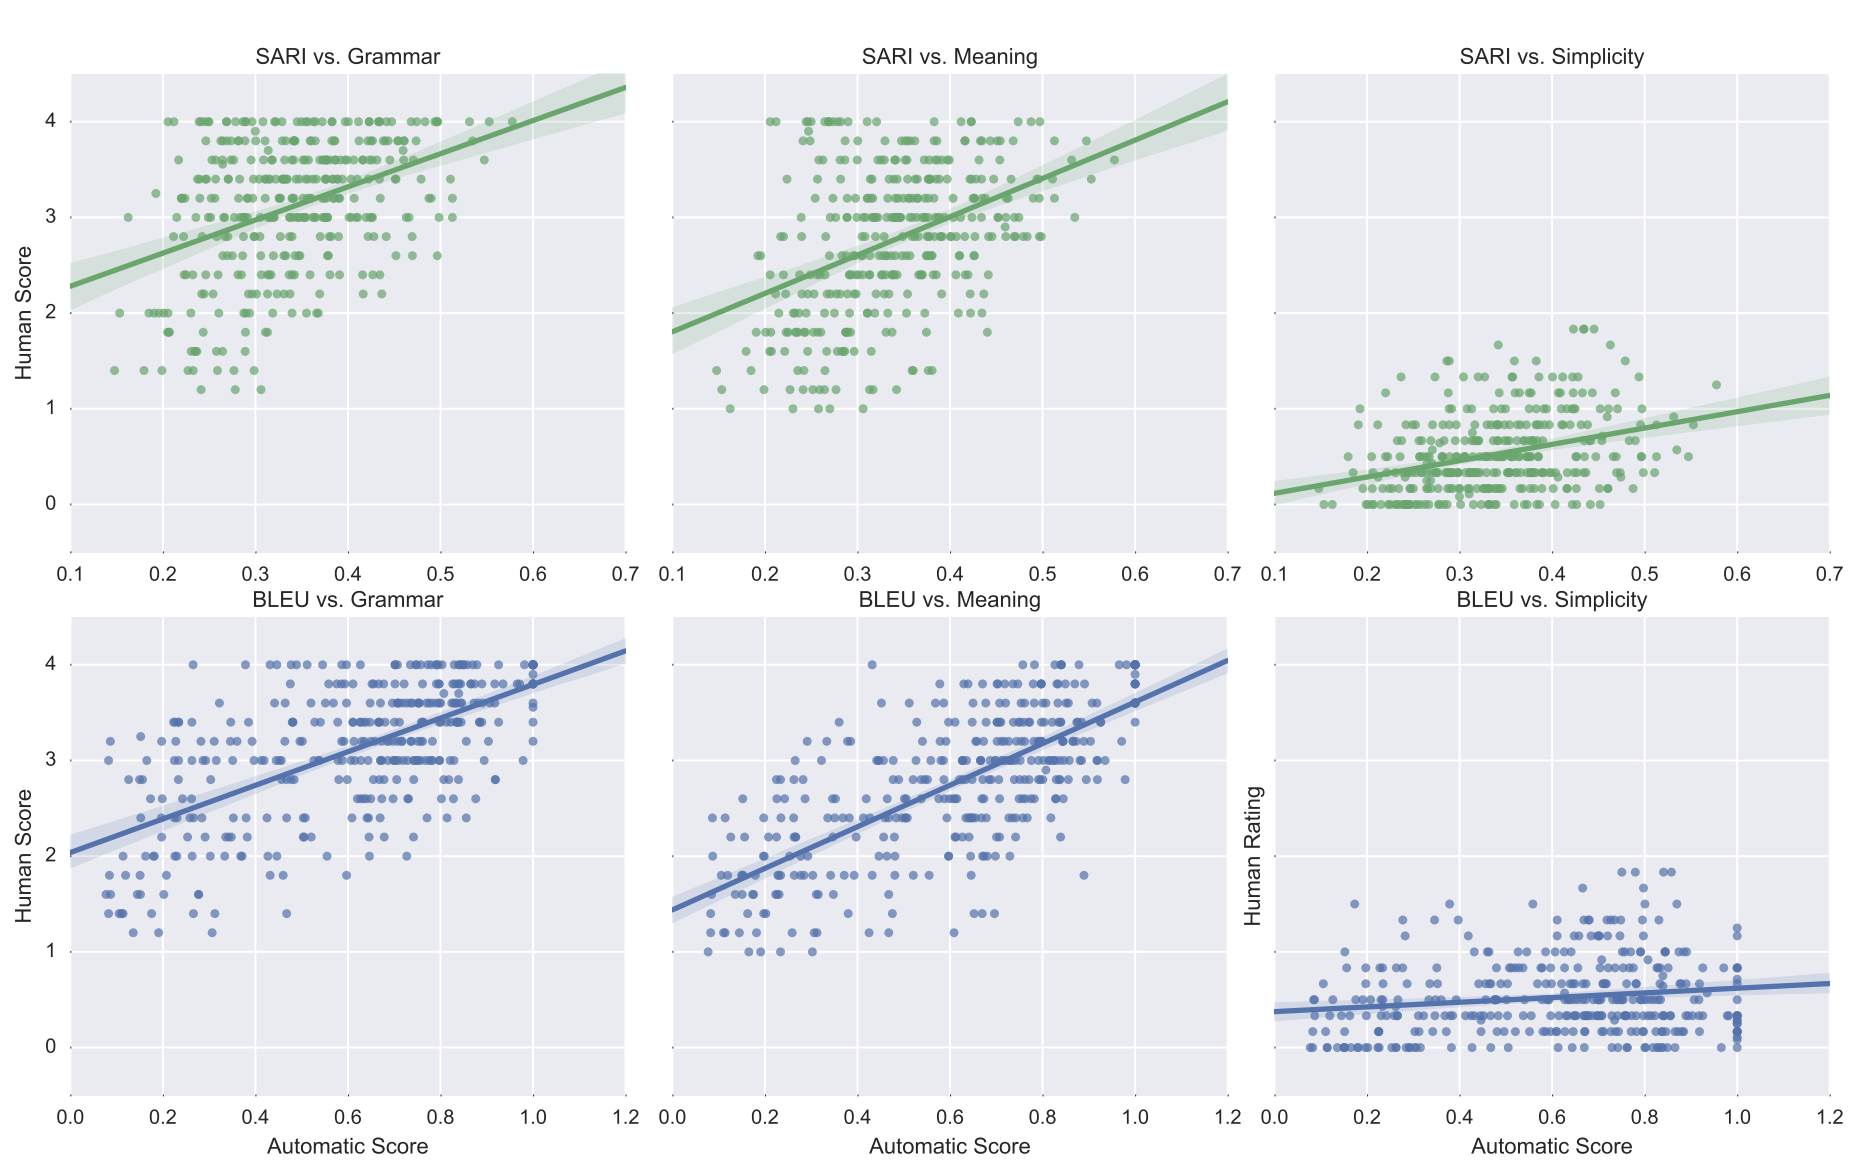
\includegraphics[width=14cm]{Images/bleu-sari.png}
    \caption{Scatter plots of automatic metrics against human scores for individual sentences. Source: \cite{xu-etal-2016-optimizing}.}
    \label{fig:bleu-sari}
\end{figure}

\bigskip
Scatter plots in fig. \ref{fig:bleu-sari} highlights the correlation of human scores on meaning and grammar with BLEU and on simplicity with SARI. The outputs which are similar to the input get a high BLEU score. That is because for the monolingual simplification task, the more references are created the more \textit{n}-grams of the input are included in the references. Outputs with few changes receive high grammar and meaning scores from humans as well, but it does not imply that they are good simplifications. Thus, BLEU prefers conservative systems that make few or no changes, while SARI penalizes them.

\section{FKGL}

Flesch-Kincaid Grade Level (FKGL) estimates the readability of text using cognitively motivated features (\cite{Kincaid1975DerivationON}). A lower value indicating higher readability. Commonly reported as measures of simplicity, FKGL relies on average sentence lengths and the number of syllables per word. Short sentences get low scores even if they have poor grammaticality or do not preserve meaning (\cite{wubben-etal-2012-sentence}). FKGL was developed by J. Peter Kincaid for the U.S. Navy in 1975. The Navy used the Flesch-Kincaid Grade score for assessing the difficulty of technical manuals.

The grade level is calculated with the following formula:

\begin{equation}
0.39\left(\frac{\#words}{\#sentences}\right)+11.8\left(\frac{\#syllables}{\#words}\right)-15.59
\end{equation}

\bigskip
A result is a number that corresponds to a US grade level. An FKGL score of 8 means that the reader needs at least a grade 8 level of reading to understand it. The FKGL coefficients were derived via multiple regressions applied to the reading compression test scores of 531 Navy personnel reading training manuals (\cite{xu-etal-2016-optimizing}). The more words a sentence contains the more difficult it is. Similarly, words with many syllables are harder to read than words that use fewer.

\section{Automatic sentence simplification evaluation}
\label{sec:easse}

\cite{alva-manchego-etal-2019-easse} introduced the \emph{Easier Automatic Sentence Simplification Evaluation} (EASSE) framework\footnote{\href{https://github.com/feralvam/easse}{https://github.com/feralvam/easse}}, a Python package for automatic evaluation of the sentence simplification. EASSE provides a broad range of evaluation resources from standard automatic metrics (e.g. BLEU, SARI, FKGL) to quality estimations and comprehensive HTML reports on quantitative and qualitative assessments of a  simplification output.

Using both the source sentence and the output simplification quality estimation, it brings additional insights into simplification systems which are not revealed by automatic metrics, e.g.: 

\begin{itemize}
    \item \emph{compression ratio}, the length of the output sentence divided by the length of the input sentence;
    \item \emph{proportion of exact matches} with the original sentences;
    \item average \emph{proportion of added words};
    \item average \emph{proportion of deleted words}.
\end{itemize}

\bigskip
In this section, we found out that the evaluation of text simplification is not a simple task and requires multiple metrics for an accurate assessment. In this work, we will use BLEU, SARI, FKGL, Exact matches ratio, Addition, and Deletion ratios. In addition, in Section \ref{sec:training-details} we introduce \textit{Compound Simplification Score} for comparing models with different BLEU, SARI and FKGL scores.


\endinput